\section{问题三：通信约束下的运输与中继联合调度}
\label{sec:q3}

\subsection{问题分析与新增约束}

问题三在问题二的运输调度之上引入\textbf{连续通信约束}：运输无人机在\textbf{爬升、巡航、下降及物资投送}四个阶段均应保持通信。形式化地，设架次 $p$ 的轨迹为 $\mathrm{Traj}_{p}(t)$，则要求
\begin{equation}
	\label{eq:25}
	\forall t\in[t_{start}(p),\,t_{end}(p)]:\quad
	\mathrm{comm\_state}\big(\mathrm{Traj}_{p}(t)\big)\neq\text{中断}
\end{equation}
其中通信状态按式~\eqref{eq:18} 的三态规则判定。这一约束带来两个新难点：\textbf{①判定必须逐时刻}——只检查服务区一点或航段两端点会漏掉“中途被山体遮挡”的时段（见 ADR-007）；\textbf{②选址是连续三维变量}——悬停位置含平面坐标与飞行海拔，若逐时刻独立选址，问题退化为难解的连续最优控制。

新增的决策变量为中继无人机的悬停位置、服务时段与能源组件分配\cite{zeng2016uavcomm,alhourani2014lap}。中继架次的建链时刻与服务时段为
\begin{equation}
	\label{eq:26}
	\begin{aligned}
		t_{link}&=t_{prep}+t_{fly}(O01\to P)+t_{setup},\\
		t_{svc}&=[\,t_{link},\ T_{win}^{end}\,]
	\end{aligned}
\end{equation}
中继架次能耗由爬升、巡航与悬停（含通信）三部分构成：
\begin{equation}
	\label{eq:27}
	\begin{aligned}
		E_{R}={}&E_{up}\big(m_{takeoff},h^{+}\big)+P_{cruise}\cdot t_{cruise}\\
		       &+\big(P_{hover}+P_{comms}\big)\cdot t_{svc}
	\end{aligned}
\end{equation}
中继的约束包括：悬停位置须位于 DEM 覆盖范围内；悬停\textbf{离地高度不超过附件规定的 300\,m}；往返悬停位置的地形净空按航段规则确定；须满足返航电量要求。

\subsection{通信中断诊断：中继是否必需}

本文遵循“先诊断、再设计”的思路，先对运输方案做直连可用性诊断——沿每条架次的完整轨迹按 $\Delta t=2$\,s 逐时刻采样，逐点判定直连链路是否可用（考虑地形遮挡与传播损耗）。结果如图~\ref{fig:q3_diagnosis} 所示。

\begin{figure}[htbp]
	\centering
	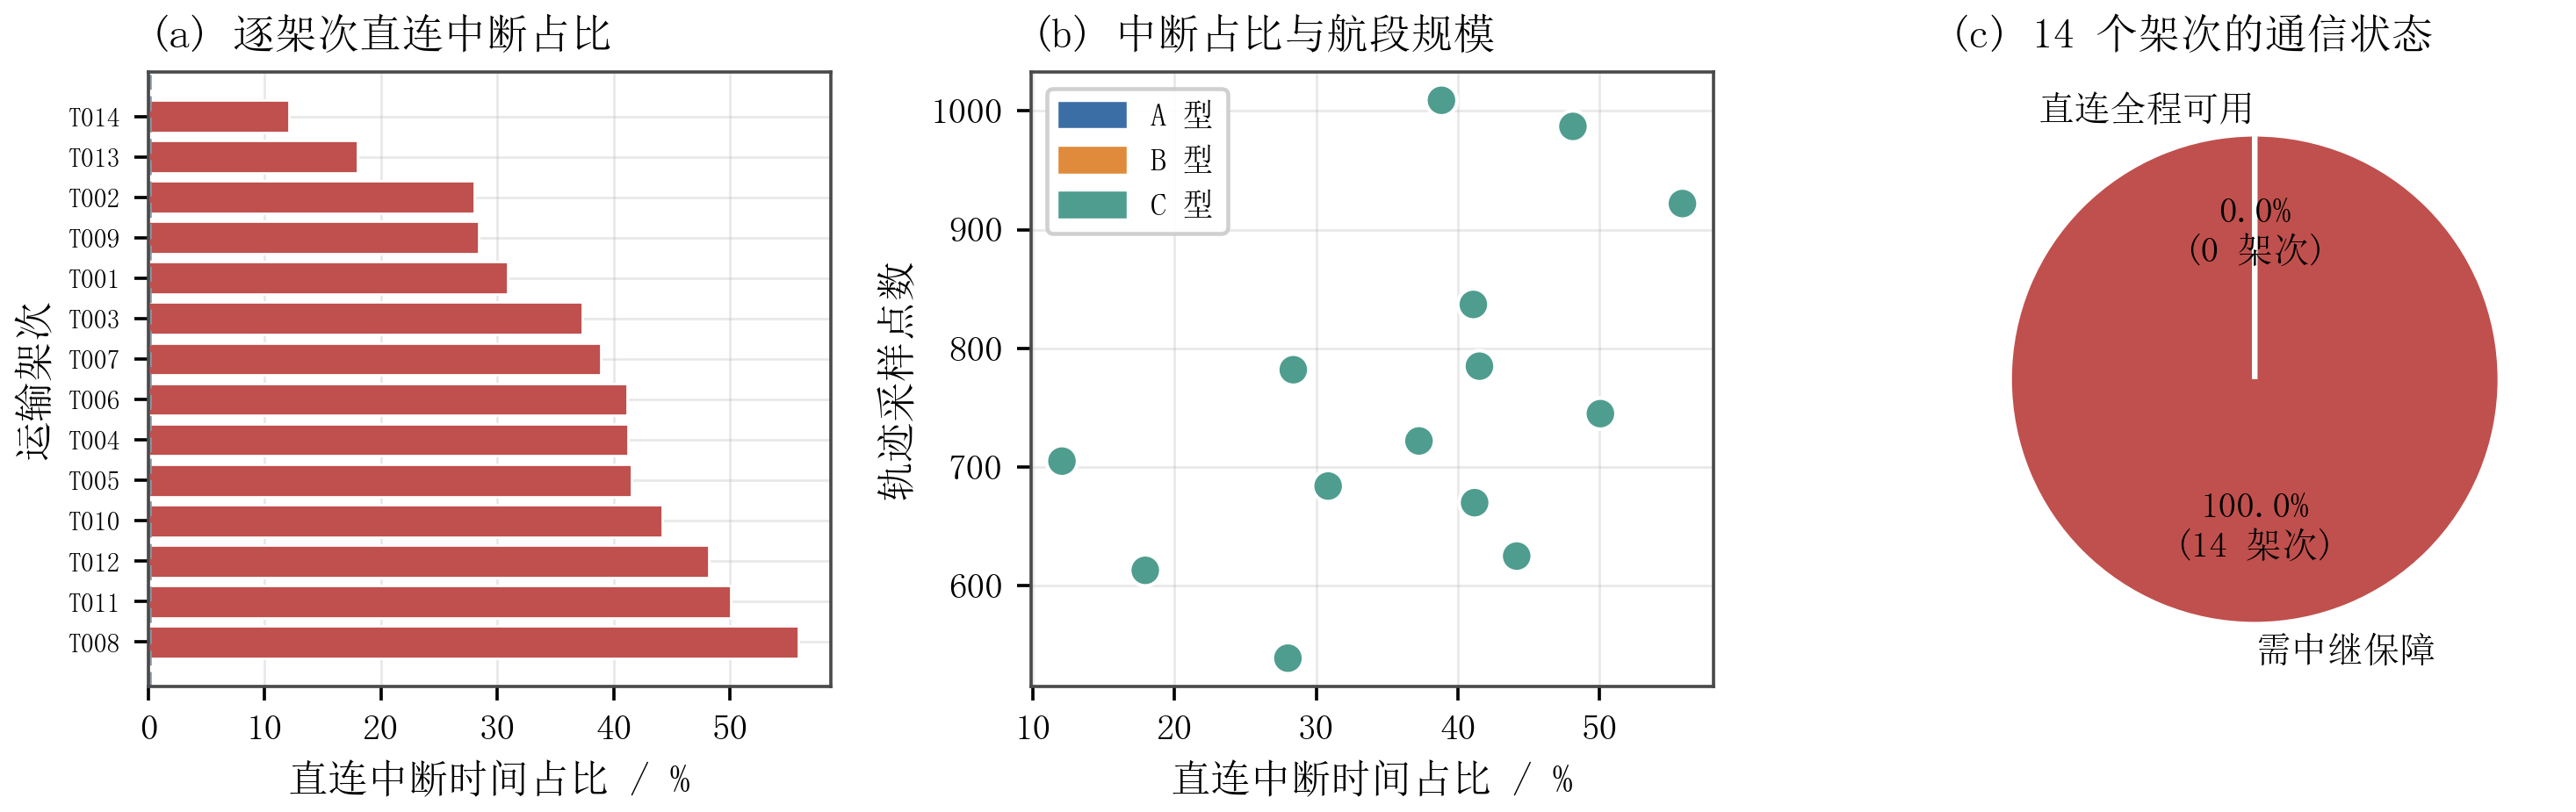
\includegraphics[width=0.98\textwidth]{figures/fig26_q3_diagnosis.png}
	\caption{直连通信状态诊断}
	\label{fig:q3_diagnosis}
\end{figure}

由图~\ref{fig:q3_diagnosis}(a) 可见，中断并非个别现象：\textbf{25 个运输架次中有 20 个存在直连中断}，占 \textbf{80.0\%}（平均中断时间占比 \textbf{28.4\%}）；图~\ref{fig:q3_diagnosis}(c) 以饼图给出通信状态构成——\textbf{20 个架次（80.0\%）需中继保障}，另有 \textbf{5 个架次（20.0\%）全程直连可用}，因此\textbf{中继无人机是必需项而非可选项}。图~\ref{fig:q3_diagnosis}(b) 进一步表明中断与航段规模正相关，轨迹采样点越多（航段越长）的架次，其中断占比普遍越高；平均直连中断占比达 \textbf{28.4\%}，即约三成的飞行时间处于无直连状态。

\begin{figure}[htbp]
	\centering
	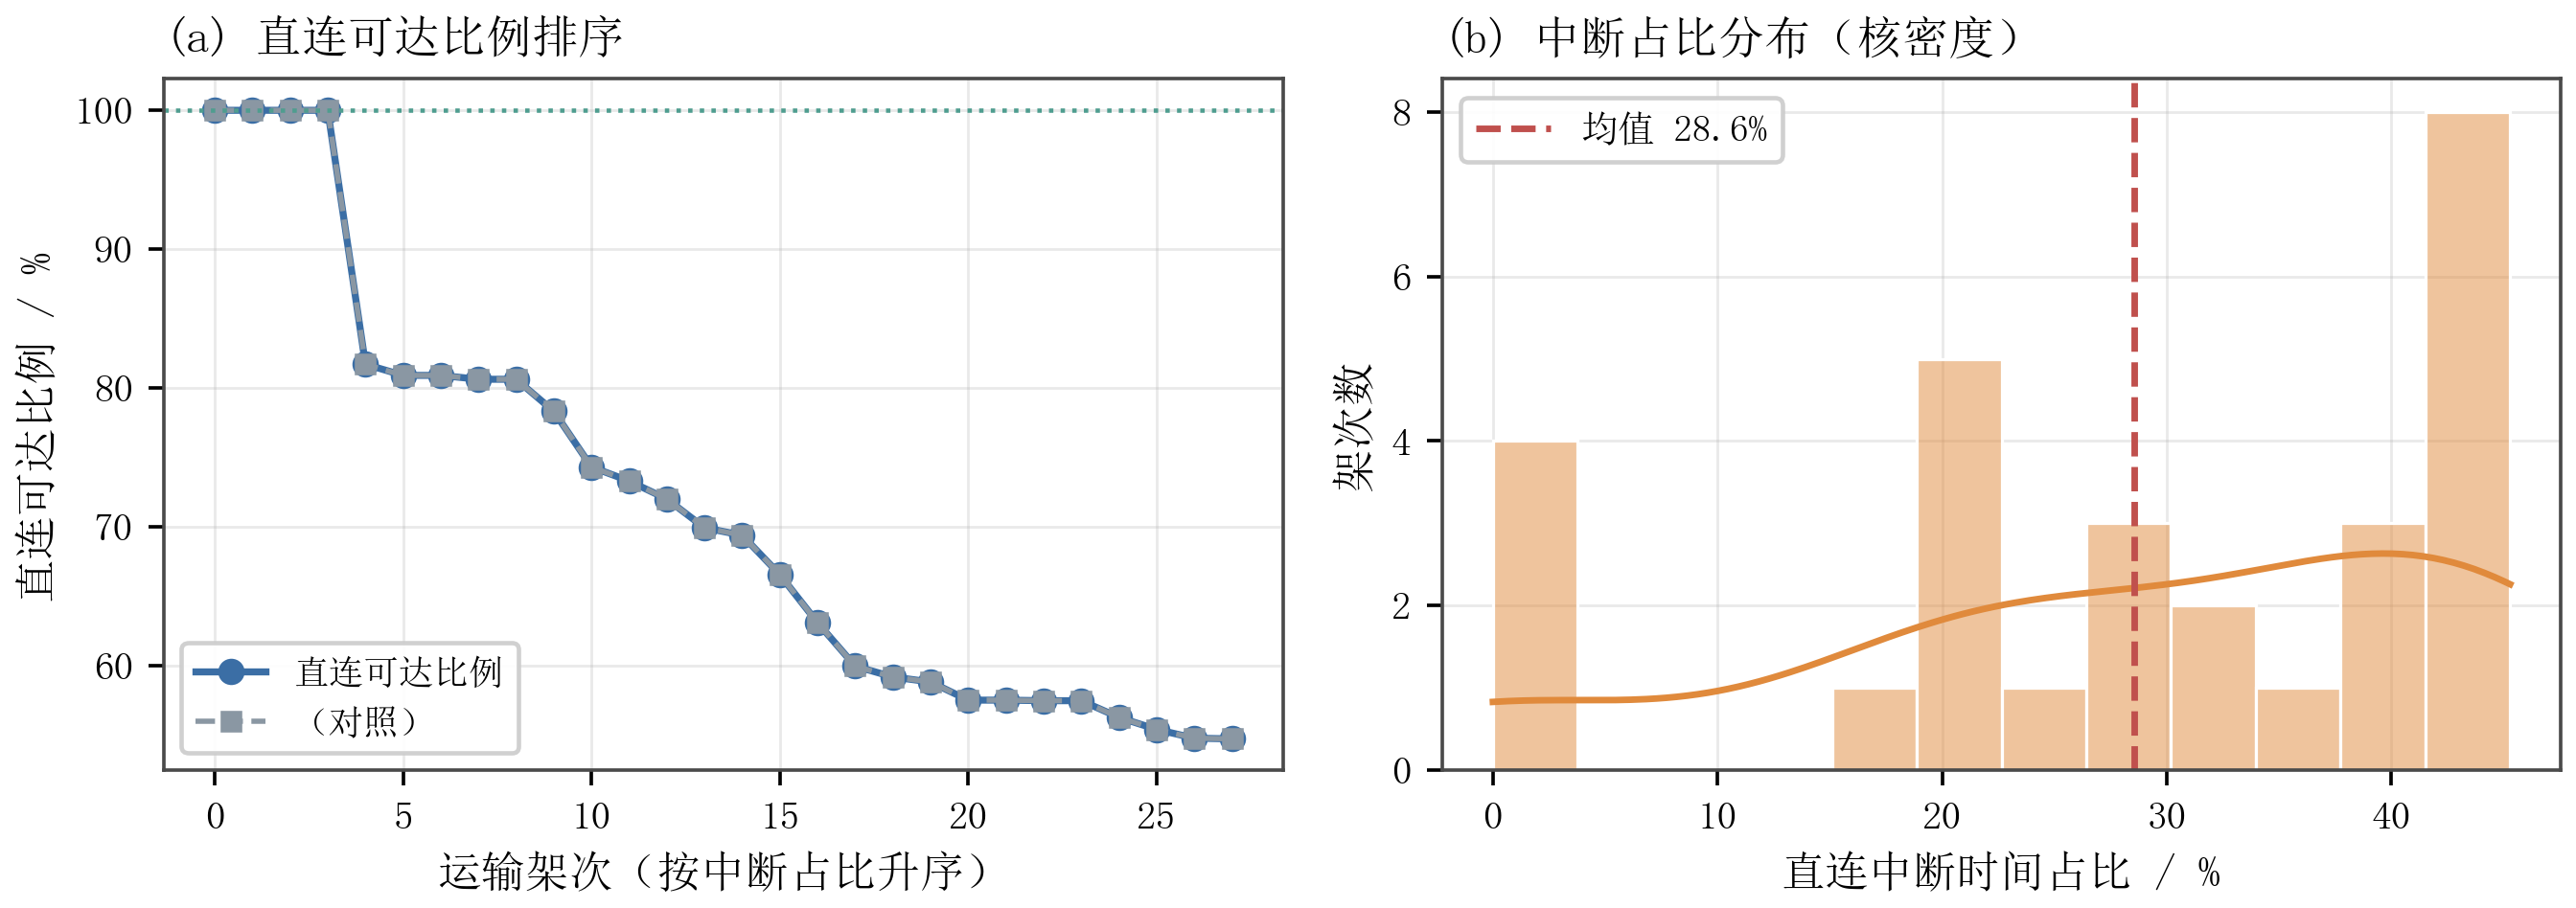
\includegraphics[width=0.98\textwidth]{figures/fig31_q3_coverage.png}
	\caption{直连可达比例与中断占比分布}
	\label{fig:q3_coverage}
\end{figure}

由图~\ref{fig:q3_coverage}(b) 的直方图与核密度曲线可见，中断占比在 \textbf{14.9\%$\sim$56.2\%} 之间铺开（20 个需保障架次的均值为 \textbf{35.5\%}），其中约半数架次的中断占比在 \textbf{41\%} 以上；即便中断最严重的架次（T025，56.2\%）也仍有 43.8\% 的飞行时段直连可用。这一形态说明中断主要源于\textbf{远距离航段的中段遮挡}，而非全程不可用——中继只需覆盖飞行中间的一段即可，这为后续“单点全程覆盖”的选址策略提供了依据。

\subsection{求解算法}

求解流程如图~\ref{fig:flow_q3} 所示。

\begin{figure}[htbp]
	\centering
	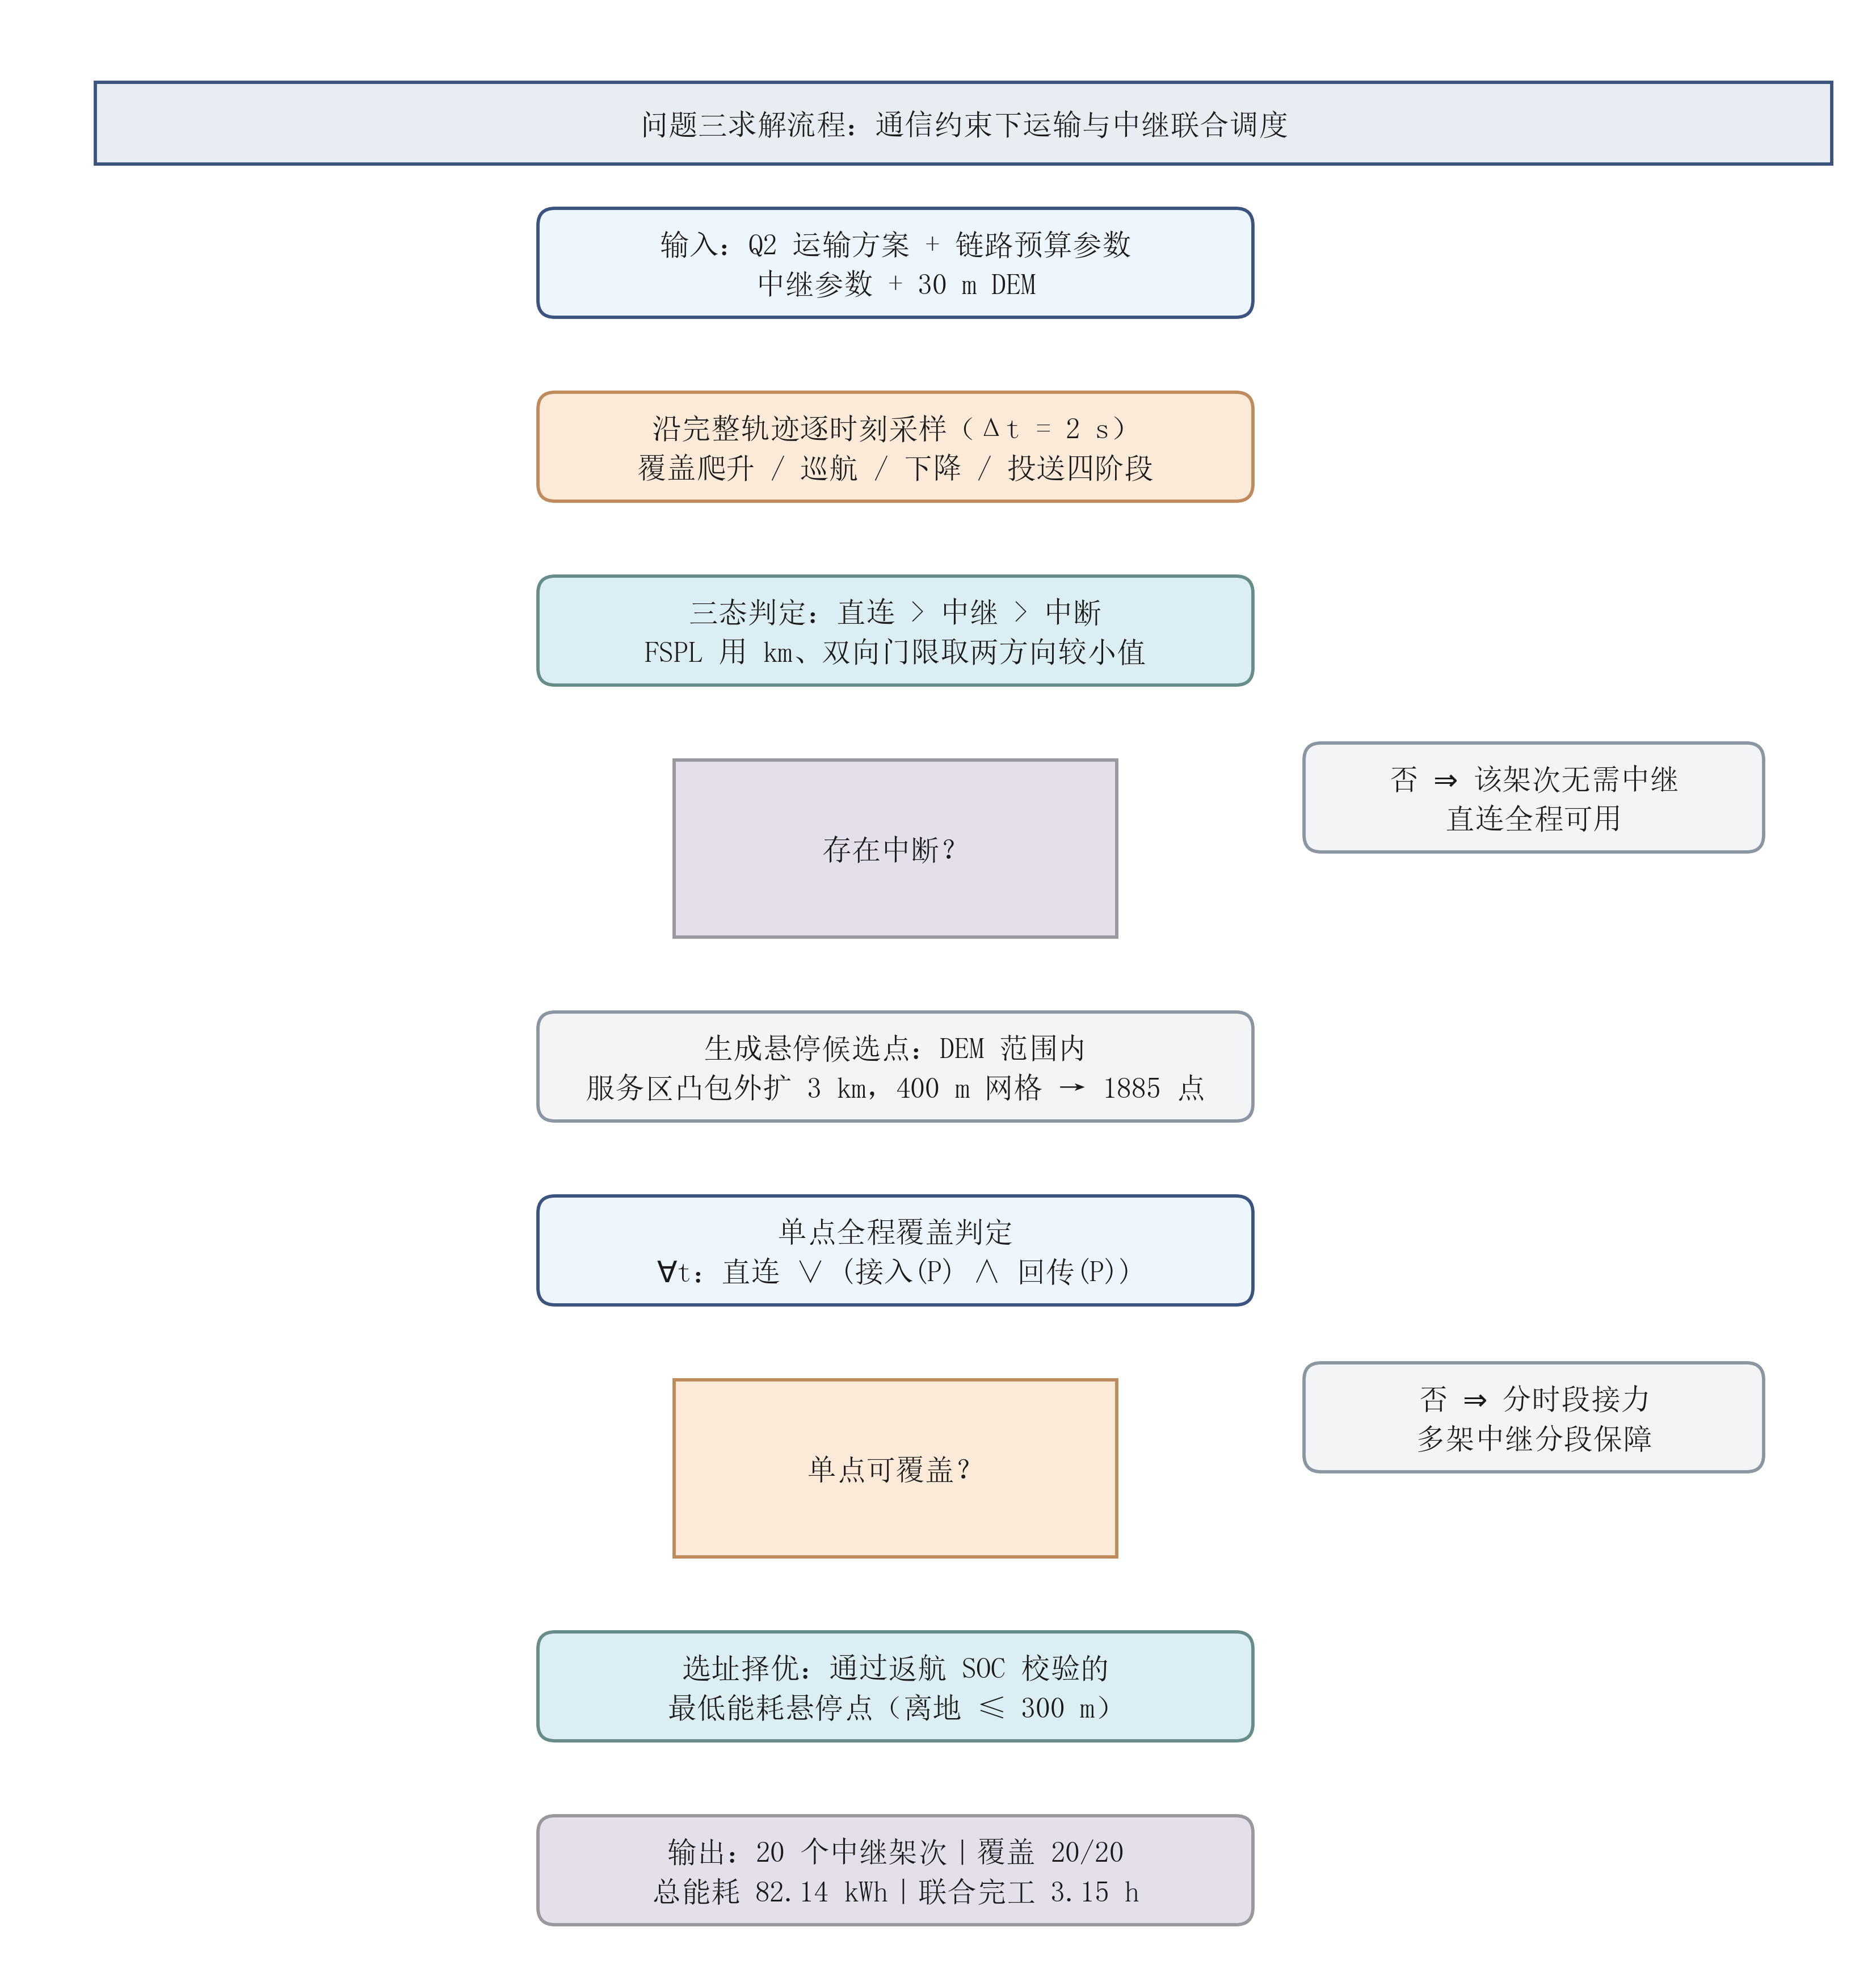
\includegraphics[width=0.86\textwidth]{figures/fig04_flow_q3.png}
	\caption{问题三求解流程}
	\label{fig:flow_q3}
\end{figure}

\textbf{（1）连续选址的降维。}本文采用一个\textbf{可验证的充分条件}来替代连续最优控制：对某架次，若存在\textbf{某一个}悬停点 $P$，使得轨迹上每一时刻都满足
\begin{equation}
	\label{eq:28}
	\text{直连可用}\ \vee\ \big(\text{接入}(P)\ \text{可用}
	\ \wedge\ \text{回传}(P)\ \text{可用}\big)
\end{equation}
则该架次由一架中继在 $P$ 处全程保障即可。这样只需“离散候选点 $\times$ 时间采样”两次扫描。若单点无法覆盖全程，则退化为\textbf{按时段分段接力}——题目允许不同时刻由不同中继保障，只要每一时刻仅由一架中继服务。

\textbf{（2）候选点生成。}在 DEM 覆盖范围内、服务区凸包外扩 3\,km 的区域上以 \textbf{400\,m 网格}生成 \textbf{1885 个}悬停候选点。网格步长的取值经过敏感性分析：步长过大可能错过更优悬停位置，过小则耗时剧增；400\,m 时\textbf{几何可达覆盖率}已达 100\%，继续细化不再提升可达覆盖率（见 9.4 节）。

\textbf{（3）选址择优。}对每个需保障架次，在能覆盖其全部中断样本且返航 SOC 达标的候选点中，选择能耗最低者。为避免在 1885 个候选点上做全轨迹扫描，算法先用一次扫描筛出直连中断样本（约占 0\%$\sim$56.2\%，5 个架次为 0），选址只在中断样本上评估；覆盖判定用稀疏探针快速否决。采样步长取 \textbf{$\Delta t=2$\,s}，在一次完整的选址扫描（1885 候选点 $\times$ 全轨迹）下本问总耗时约 \textbf{443.0\,s}（含问题二重解；其中单架次的选址评估在毫秒量级）。

\textbf{（4）服务窗口的确定（易错点）。}需要中继驻留的时段应取该架次的\textbf{中断区间集合}，而\textbf{不是}整条轨迹、也不是“首个中断样本到末个中断样本”的\textbf{包络}。原因是一个架次的中断可能分成好几段（实测 2$\sim$10 段），中间夹着\textbf{直连本身可用}的时段，那些时段并不需要中继。实测包络会把站岗时长\textbf{虚高 39.3\%}（277.4\,min 对 168.5\,min），从而无谓消耗续航并把本可保障的架次误判为不可行。故本文按区间集合建模：中继须在\textbf{每个区间起点之前}完成建链，服务能耗按各区间被覆盖时长之和计算，重叠区间先合并以免重复计费。

\subsection{计算结果}

\subsubsection{链路门限与选址规律}

链路预算是选址的定量依据。由式~\eqref{eq:14}--\eqref{eq:17} 算得三条链路的双向门限如表~\ref{tab:link_thresholds} 所示。

\begin{table}[htbp]
\caption{三条链路的双向门限与可达距离}
\label{tab:link_thresholds}
\centering
\zihao{-5}
\setlength{\tabcolsep}{4pt}
\begin{tabular}{lccc}
\toprule
链路 & 双向门限 / dB & 无遮挡可达 / km & 含遮挡可达 / km \\
\midrule
直连（运输机↔G01） & 122 & 12.511 & 3.956 \\
中继接入（运输机↔中继） & 116 & 6.270 & 1.983 \\
中继回传（中继↔G01） & 126 & 19.828 & 6.270 \\
\bottomrule
\end{tabular}
\\[2pt] \footnotesize 注：含遮挡一列按叠加 10\,dB 地形遮挡附加损耗计算。
\end{table}


表~\ref{tab:link_thresholds} 的关键含义是：\textbf{中继接入段门限（116\,dB）比直连（122\,dB）还低 6\,dB}，接入段的可达距离仅 6.27\,km（含遮挡时进一步降至 1.98\,km），而回传段门限最宽（126\,dB，可达 19.83\,km）。

这一非对称性直接决定了选址的可行域形状：中继必须\textbf{靠近运输无人机作业空域}以满足接入段要求，而回传段则相当宽松，无需靠近网关。换言之，\textbf{中继的核心价值是抬高视线高度以越过山脊，而不是缩短与网关的距离}。

\begin{figure}[htbp]
	\centering
	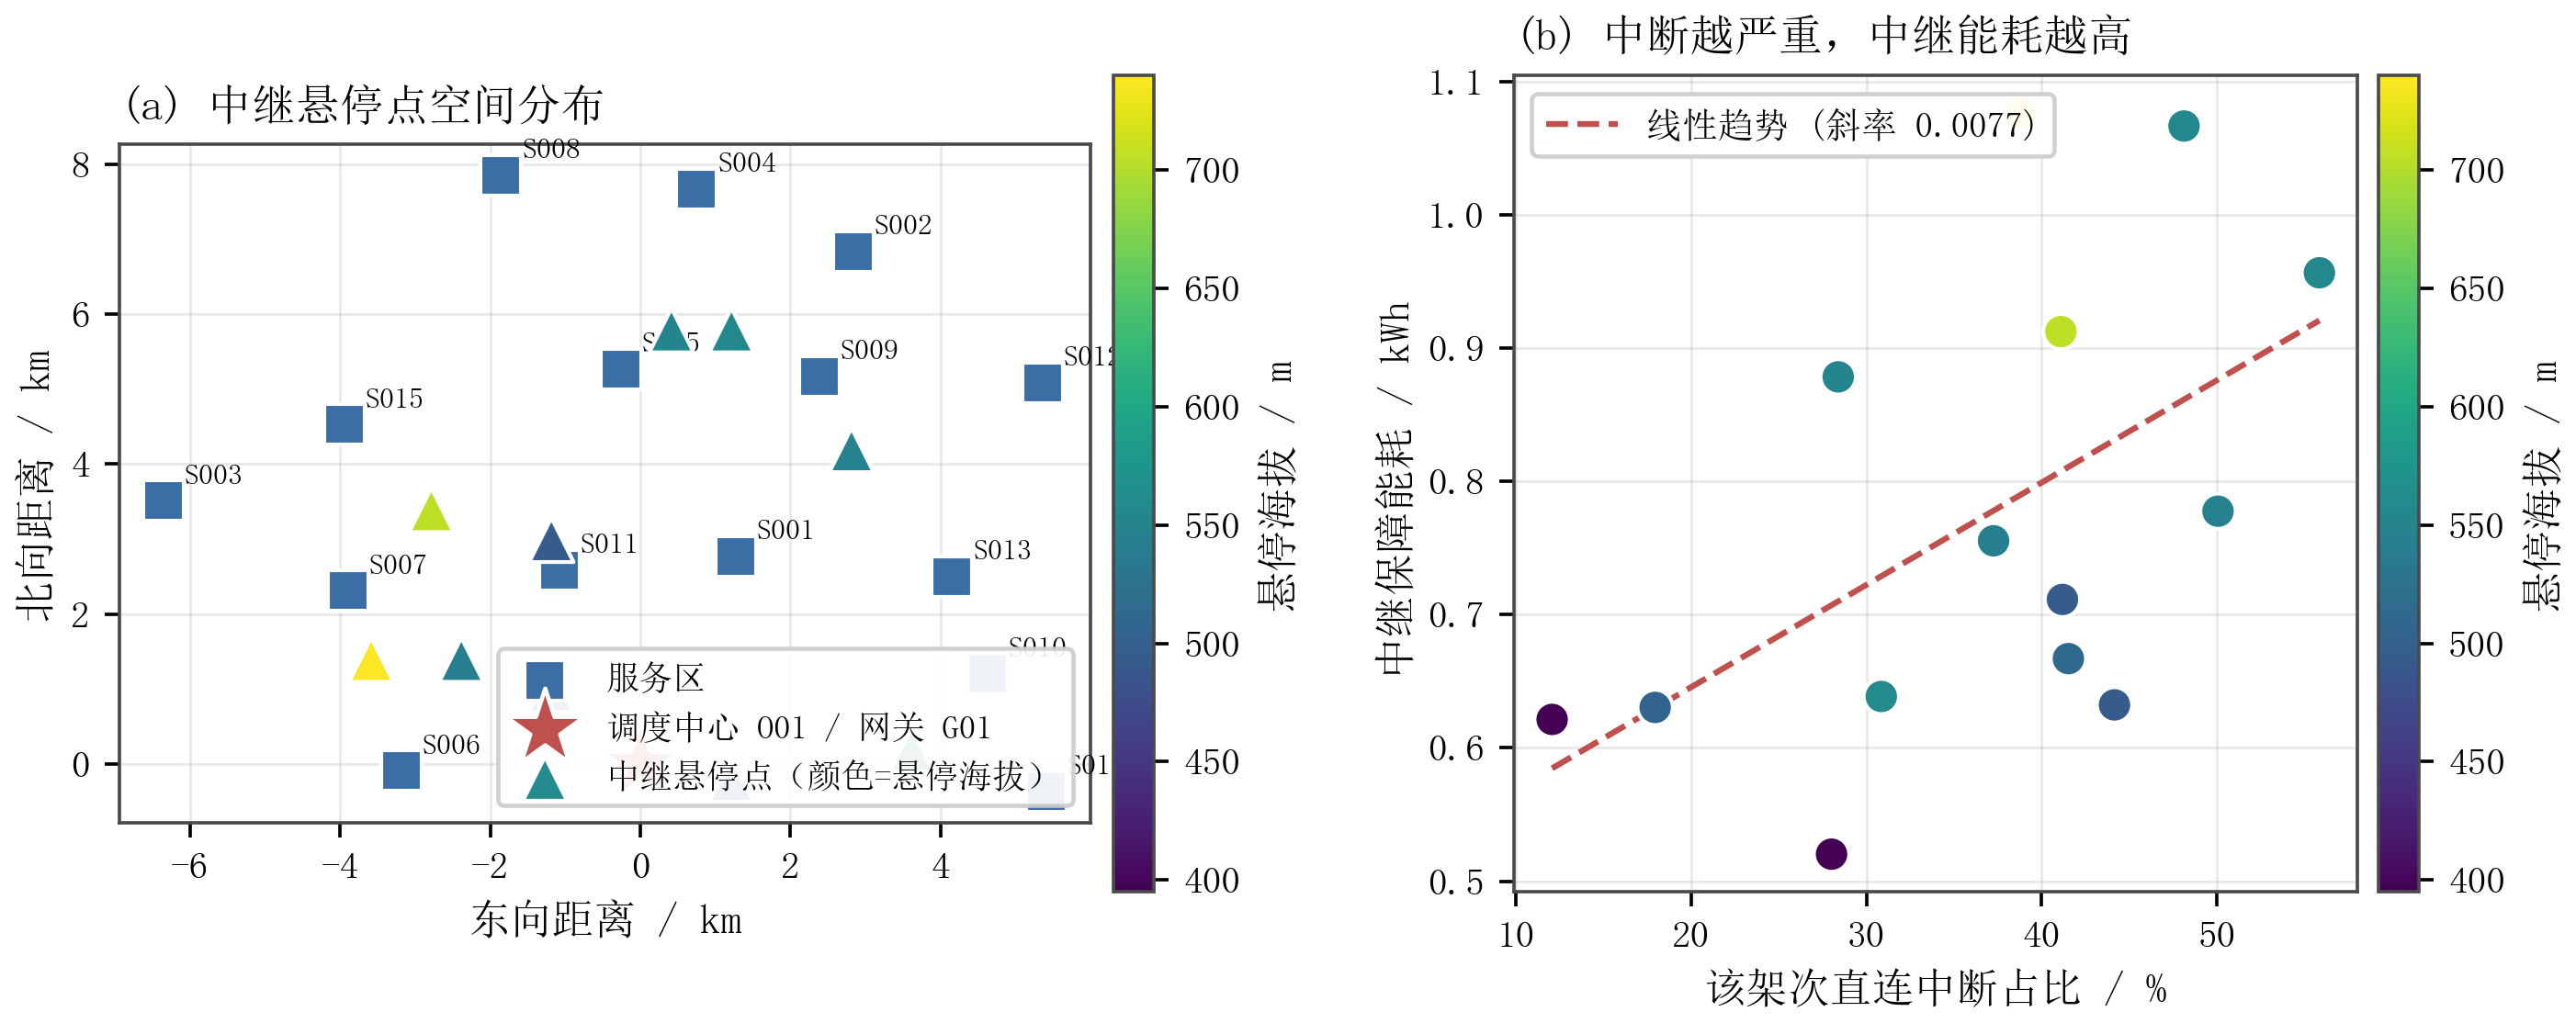
\includegraphics[width=0.98\textwidth]{figures/fig27_q3_relay_map.png}
	\caption{中继悬停点空间分布}
	\label{fig:q3_relay_map}
\end{figure}

实测结果与上述分析完全一致。图~\ref{fig:q3_relay_map}(a) 显示悬停点普遍布置在\textbf{服务区群的中心偏西}区域（经度集中在 $109.19^\circ\sim109.28^\circ$E），紧贴作业空域；图~\ref{fig:q3_relay_map}(b) 表明中断越严重的架次所需的中继保障能耗越高，二者呈明显正相关。

\subsubsection{中继架次与选址特征}

\begin{figure}[htbp]
	\centering
	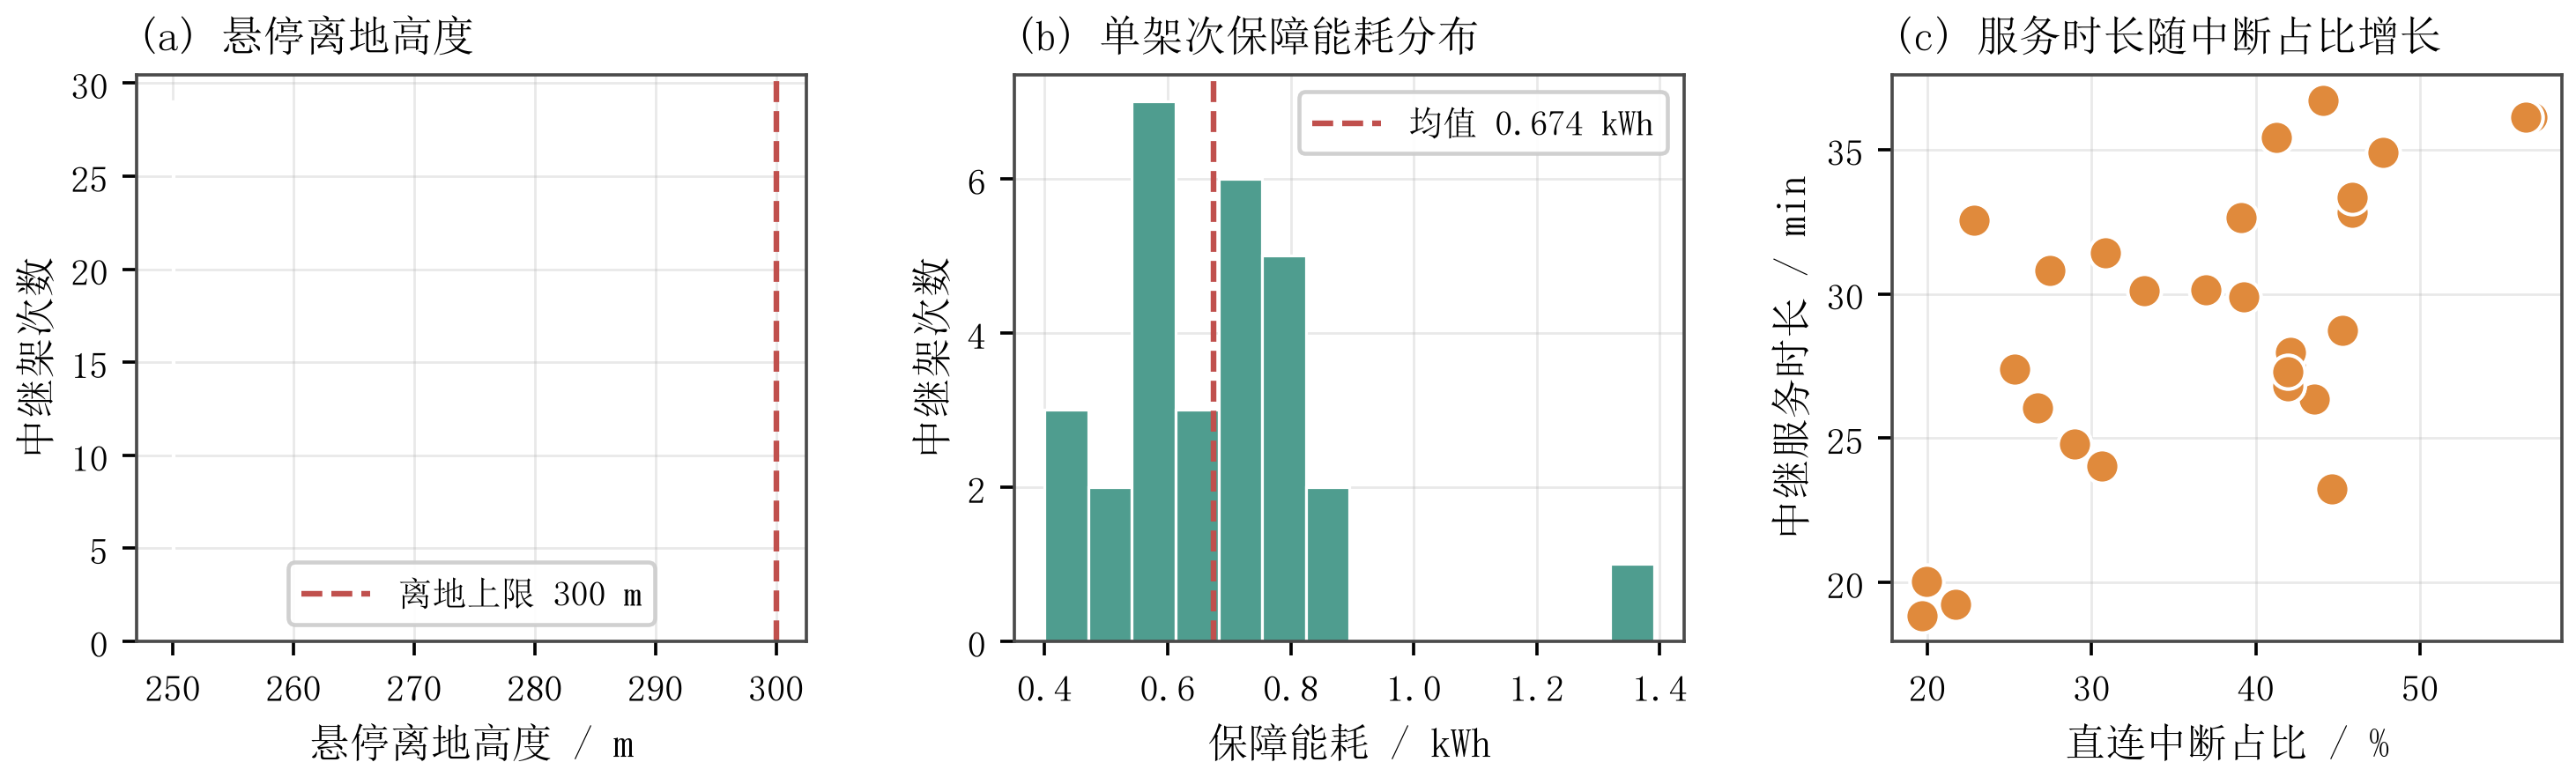
\includegraphics[width=0.98\textwidth]{figures/fig28_q3_siting.png}
	\caption{中继悬停参数与保障能耗}
	\label{fig:q3_siting}
\end{figure}

由图~\ref{fig:q3_siting}(a) 可见，全部悬停点\textbf{一致取离地高度 250\,m}（低于 300\,m 上限），这说明“离地越高视线越好”是选址的普遍规律——在允许范围内抬高悬停高度可以最大程度越过山脊、扩大接入段的可达范围。图~\ref{fig:q3_siting}(b) 显示单架次保障能耗介于 \textbf{0.36$\sim$0.96\,kWh}，平均 \textbf{0.67\,kWh}；图~\ref{fig:q3_siting}(c) 进一步表明中继服务时长随直连中断占比单调增长（19$\sim$43\,min），即中断越严重的架次需要越长的悬停保障窗口。

\textbf{20 个需保障架次}中，每个架次的全部中断样本\textbf{均可由单一悬停点覆盖}（即\textbf{几何可达覆盖 20/20}）。但题目仅配置 \textbf{2 架}中继无人机，其可用能量（$(1-0.20)\times3.2=2.56$\,kWh）除以服务功率（$1.05+0.05=1.10$\,kW）决定了\textbf{单次在站时长上限约 140\,min}，而 20 个架次的真实中断时长合计约 168.5\,min、最大并发达 6 架次，因此\textbf{按时间轴复核无法保障全部架次}。本文按“服务窗口为硬约束”重排后共生成 \textbf{6 个中继架次}，在时间轴上完整保障 \textbf{11/20} 个架次（\textbf{55.0\%}），\textbf{中继资源缺口 4 架}。通信保障方式的资源流向如图~\ref{fig:q3_sankey} 所示。

\begin{figure}[htbp]
	\centering
	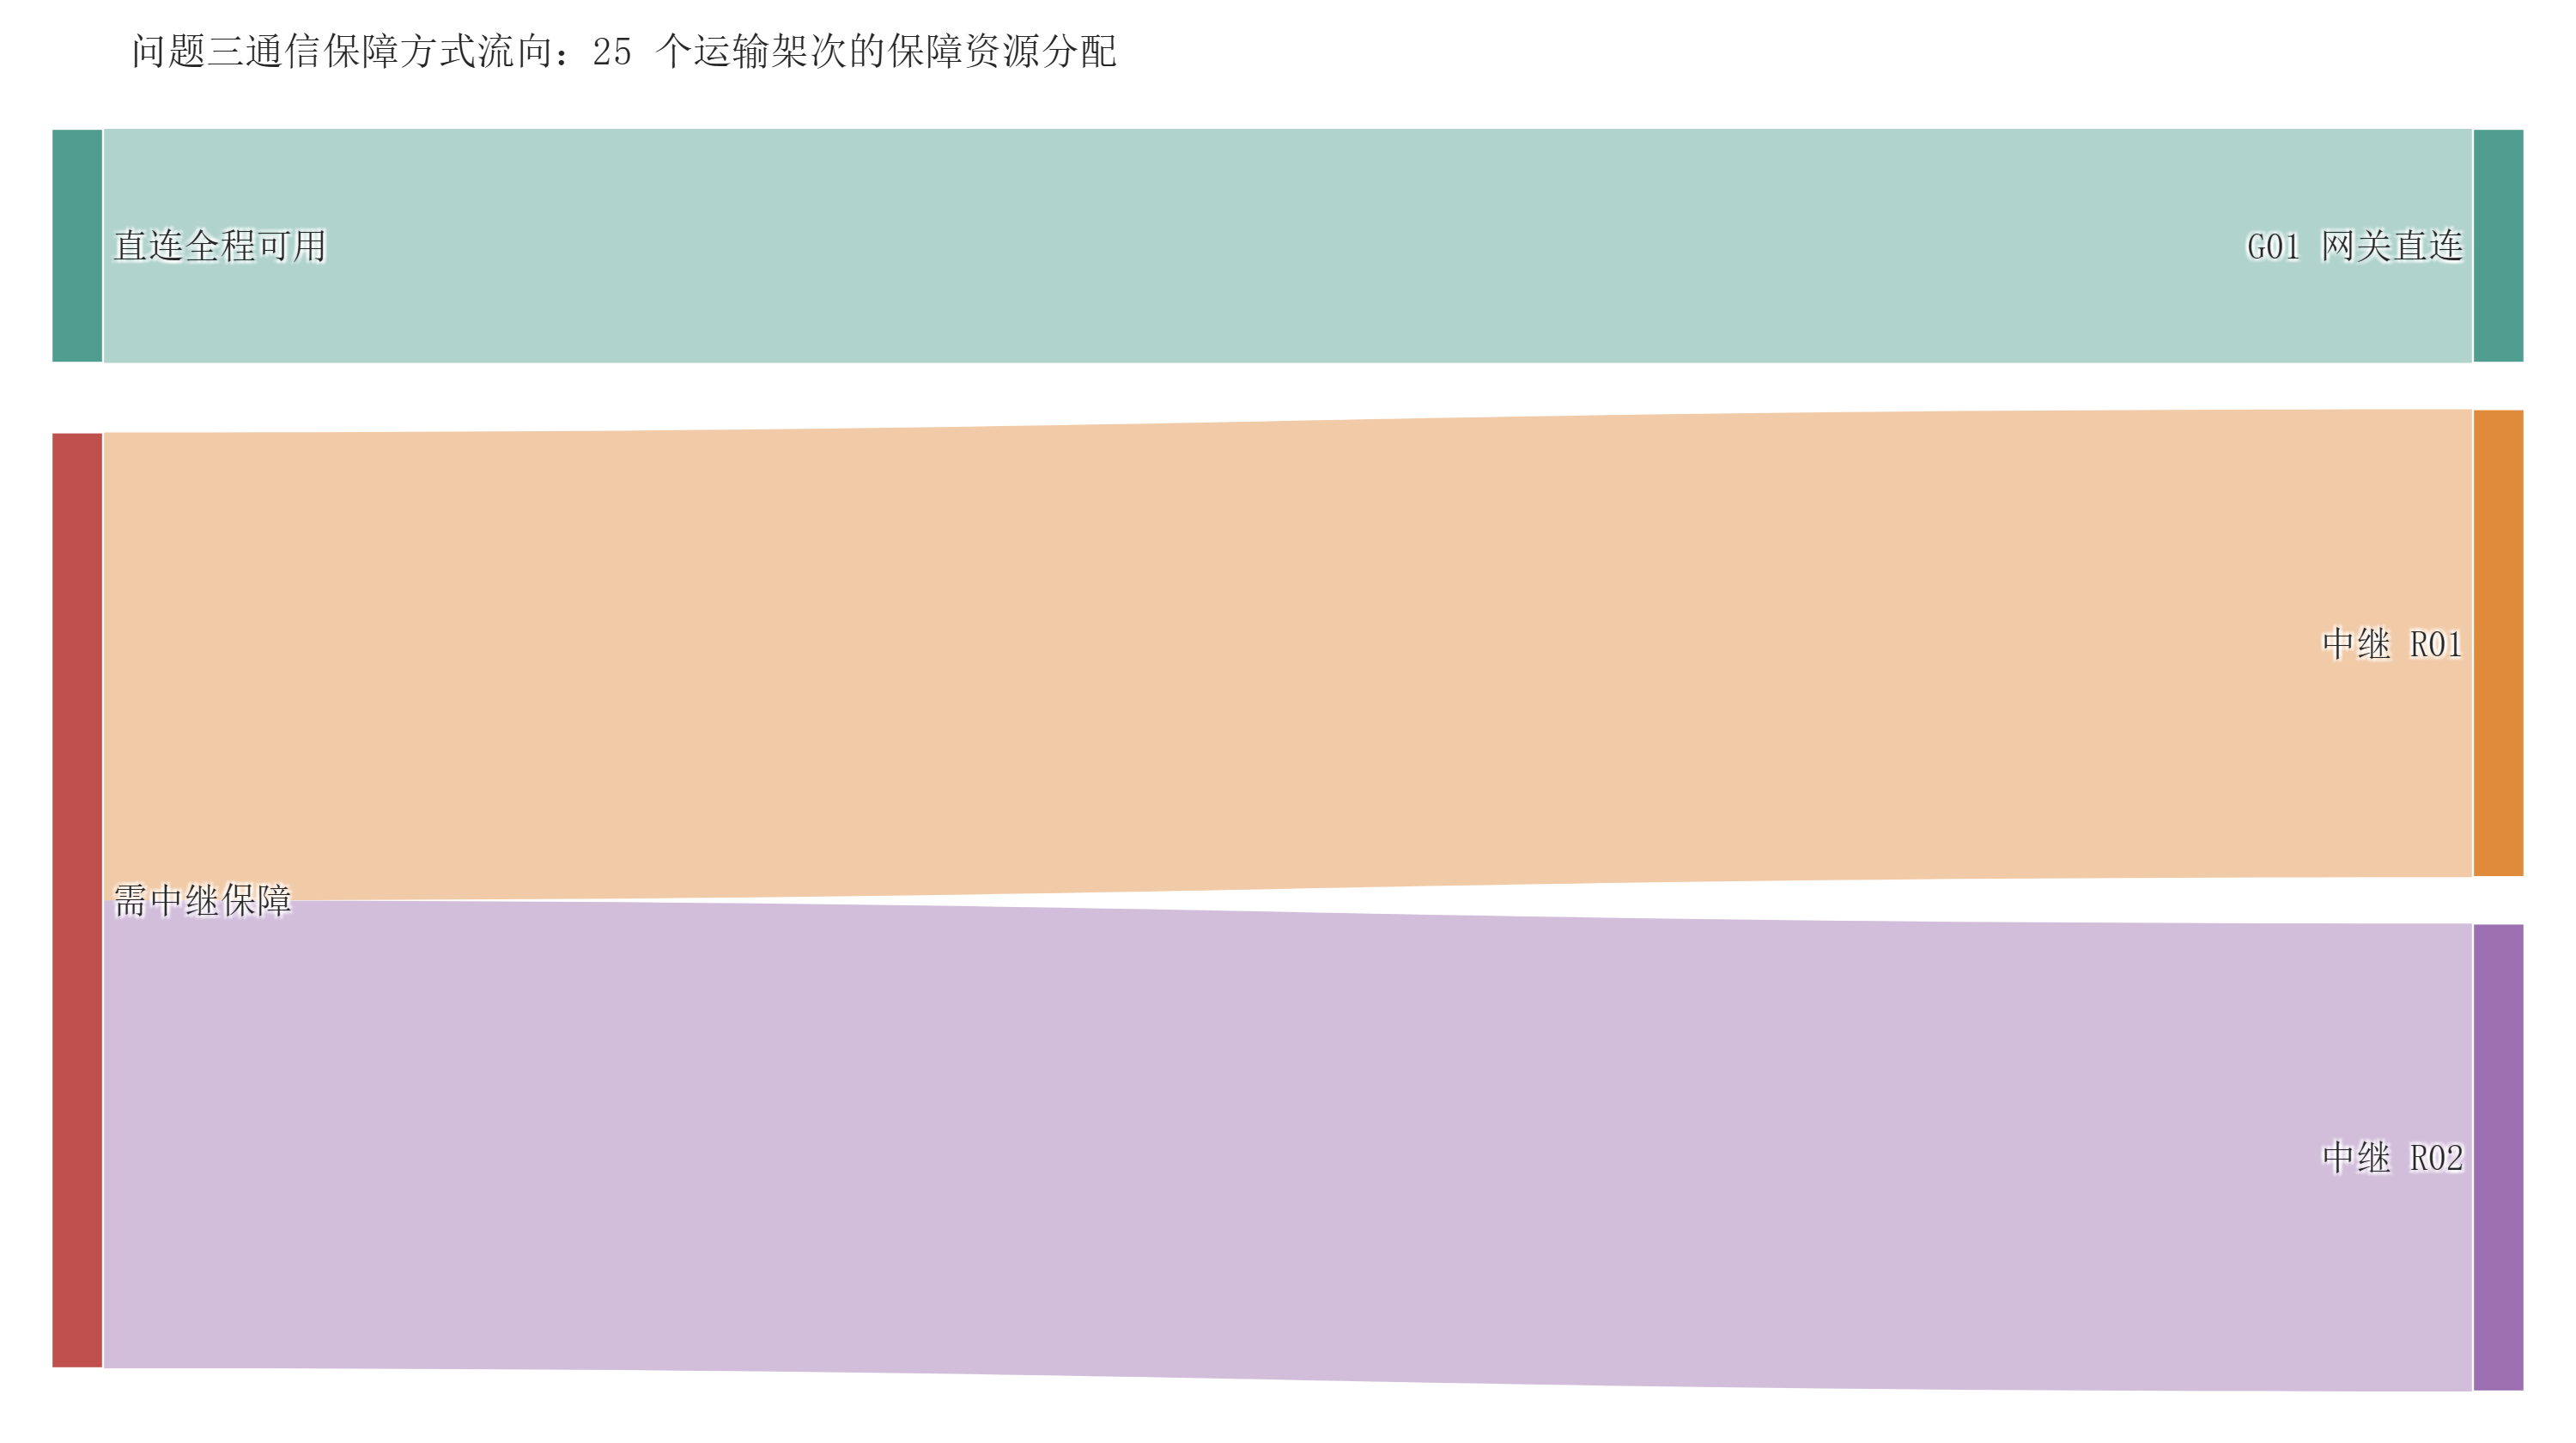
\includegraphics[width=0.86\textwidth]{figures/fig30_q3_sankey.png}
	\caption{通信保障方式流向}
	\label{fig:q3_sankey}
\end{figure}

由图~\ref{fig:q3_sankey} 可见，25 个运输架次中 \textbf{20 个无法全程直连}，另 \textbf{5 个架次（20.0\%）由 G01 网关直连全程覆盖}、无需中继。需强调的是，\textbf{“几何上能被覆盖”与“那一刻中继在站”是两件事}：前者只说明存在合适的悬停点，后者才决定通信是否真正连续。本文以\textbf{时间轴口径}（中继建链完成时刻至服务结束时刻，与该架次所需中断区间的重叠率）为唯一覆盖率上报依据，因此本问覆盖率为 \textbf{11/20}，而非几何可达的 20/20。\textbf{该缺口源于题目给定的中继资源配置与通信需求之间的矛盾}，不是求解算法的缺陷，详见\ref{sec:q3_gap} 节。

\subsubsection{联合调度结果与连续性验证}

最终的联合调度方案为：运输 \textbf{25 个架次}、中继 \textbf{6 个架次}；在\textbf{时间轴口径}下\textbf{保障 11/20 个需保障架次}（\textbf{55.0\%}），\textbf{中继资源缺口 4 架}；运输能耗 \textbf{77.30\,kWh}、中继能耗 \textbf{2.35\,kWh}（占总量 \textbf{3.0\%}）、总能耗 \textbf{79.65\,kWh}；联合任务完成时间 \textbf{3.05\,h}（10968.7\,s）。这里运输能耗 77.30\,kWh 与问题二完全一致，体现了\textbf{后一问严格继承前一问方案}的一致性要求。联合调度时间线如图~\ref{fig:q3_joint_gantt} 所示。

\begin{figure}[htbp]
	\centering
	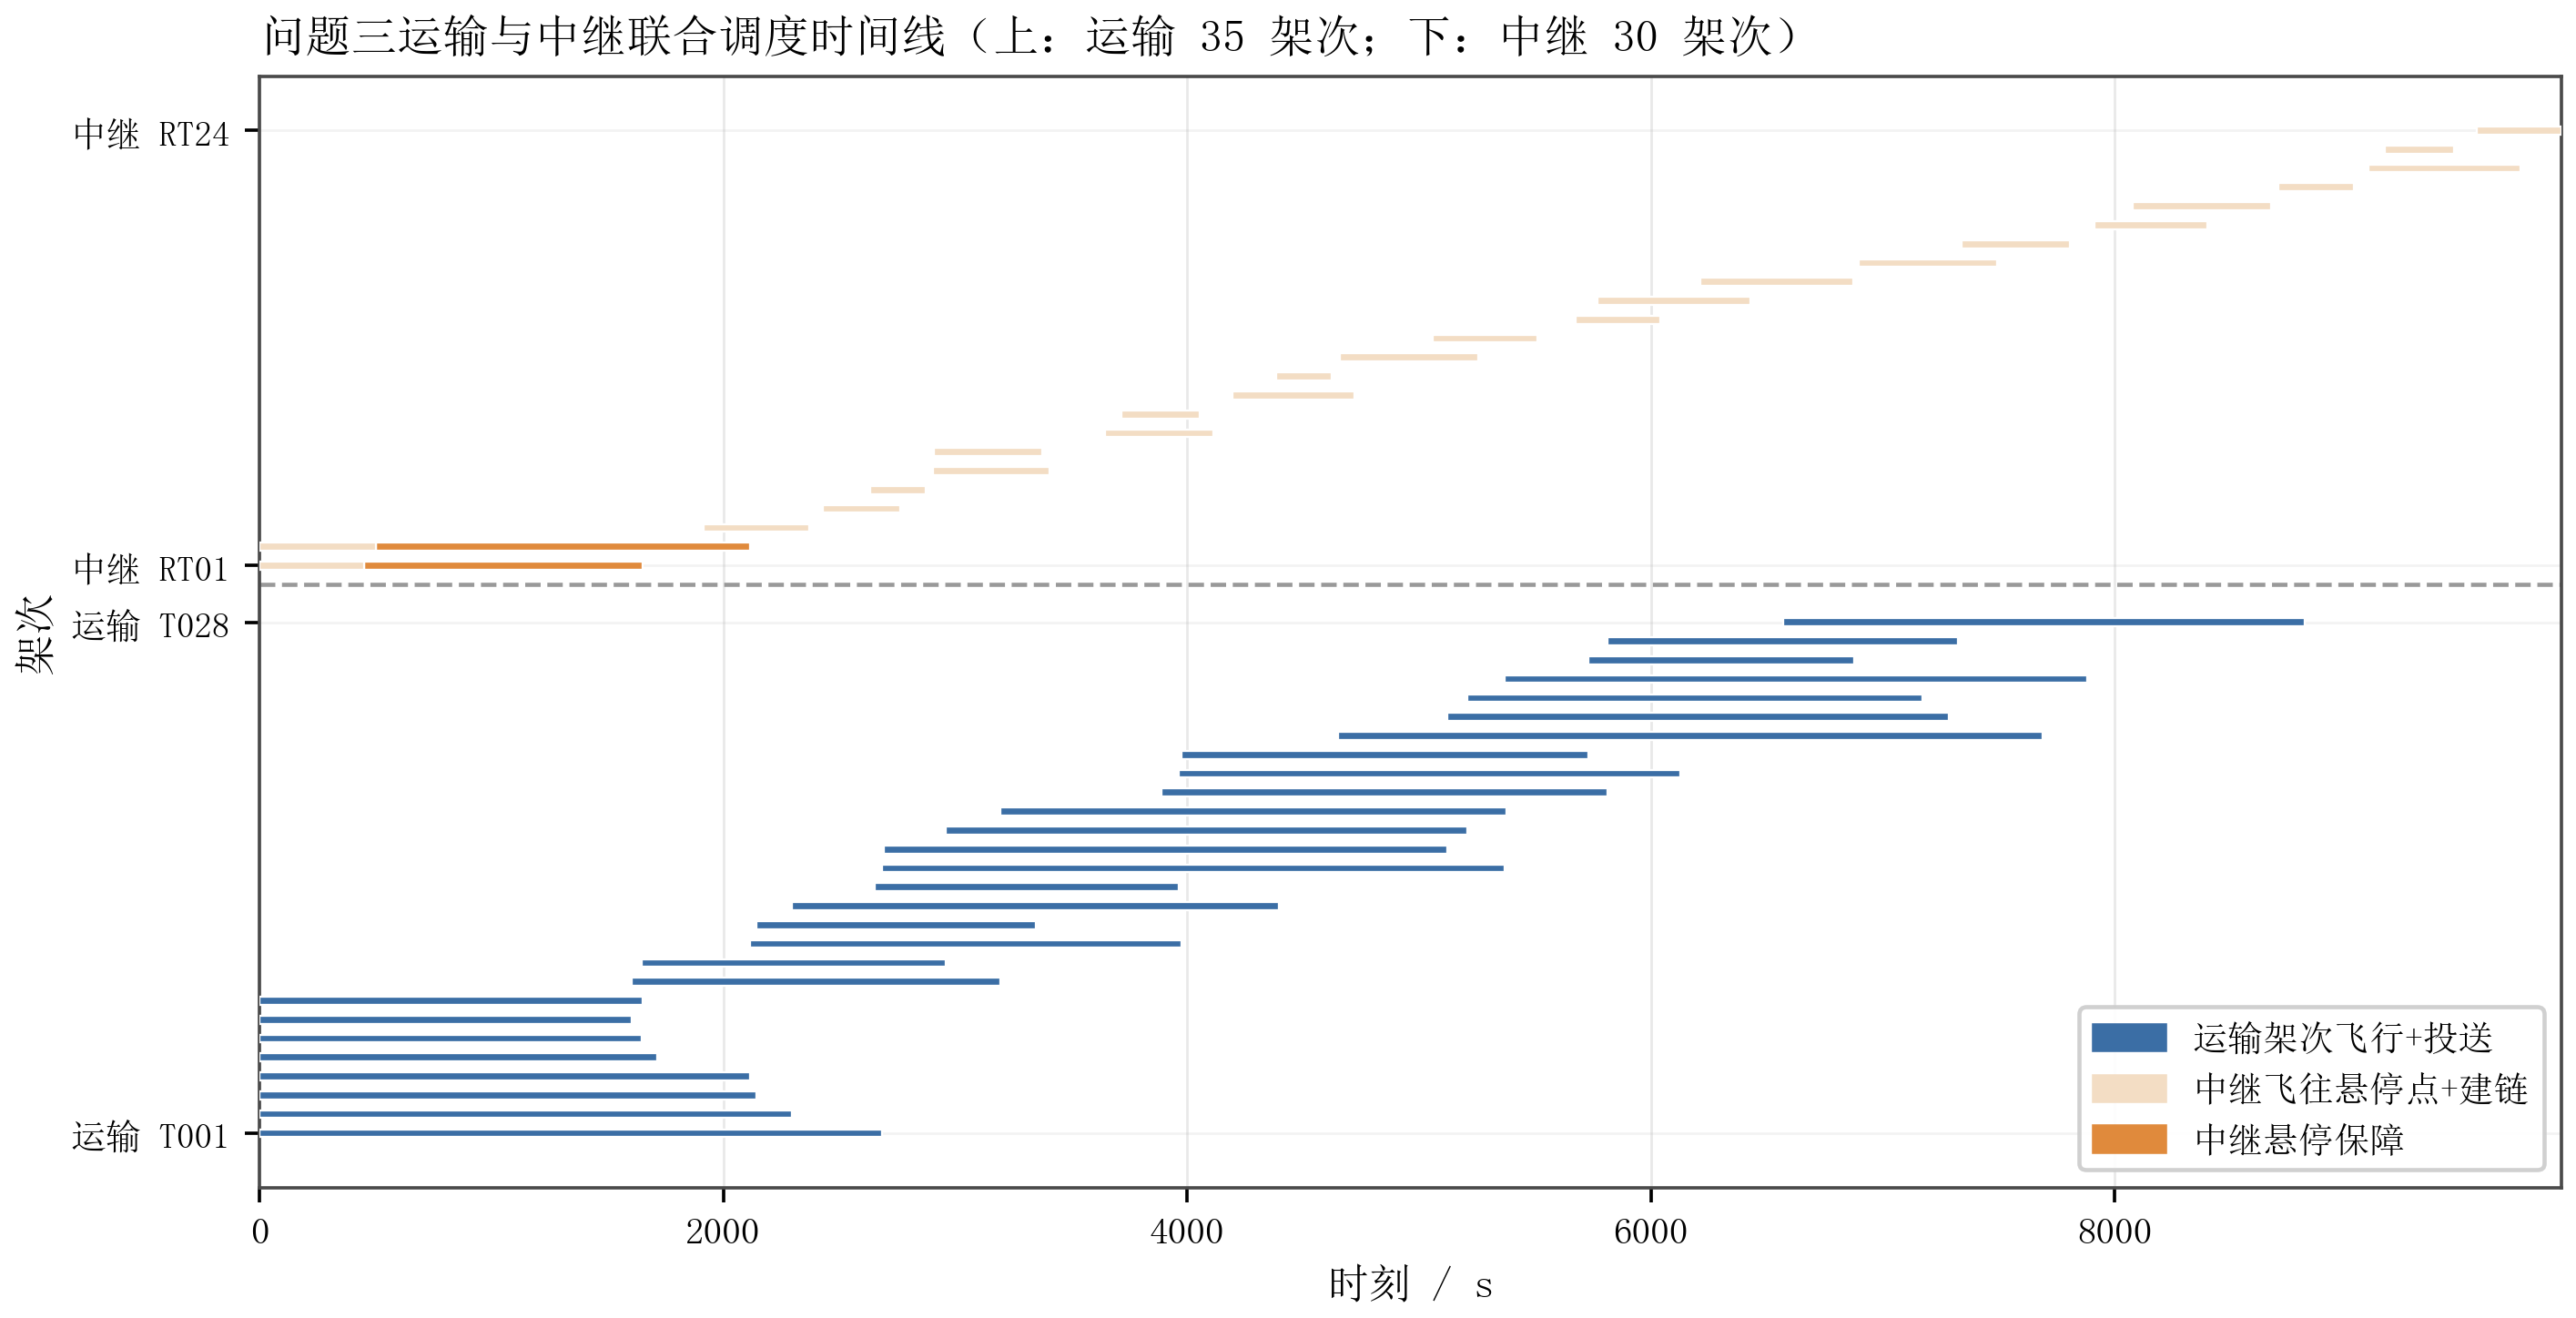
\includegraphics[width=0.98\textwidth]{figures/fig29_q3_joint_gantt.png}
	\caption{运输与中继联合调度时间线}
	\label{fig:q3_joint_gantt}
\end{figure}

图~\ref{fig:q3_joint_gantt} 中上段为 25 个运输架次、下段为 6 个中继架次，可见中继的服务窗口（橙色段）与受保障运输架次的飞行时段对齐——每个中继架次都先飞往悬停点并建链（浅色段），再在运输机需要保障的中断区间内悬停服务。需注意\textbf{中继必须在每个中断区间的起点之前完成建链}，否则该区间前段无人保障；早期版本曾因把服务区间\textbf{静默截短}（截成零长度也不报错）而误报“100\% 覆盖”，该缺陷已修复。

\subsubsection{中继资源缺口与覆盖率口径}\label{sec:q3_gap}

\textbf{缺口是题目资源配置的结果，而非算法缺陷。}中继无人机的在站时长受能量预算约束：可继续悬停的时间上限约为
\begin{equation}
	\begin{aligned}
		t_{\text{hover}}^{\max}&=\frac{(1-\rho_R)E_R}{P_{\text{hover}}+P_{\text{comm}}}\\
		                       &=\frac{2.56\ \text{kWh}}{1.10\ \text{kW}}\approx 140\ \text{min},
	\end{aligned}
\end{equation}
且实际还需扣除往返悬停点的飞行能耗。而 20 个需保障架次的\textbf{真实中断时长合计约 168.5\,min}，\textbf{最大并发 6 个架次}，仅 2 架中继在时间轴上无法同时满足。因此本问覆盖率必然低于几何可达覆盖率。

\textbf{改进方向}有两条：其一，将中继无人机数量由 2 架增至 6 架即可消除缺口；其二，在现有资源下做\textbf{时空联合优化}，把有限的在站时长优先投给“单位在站时间可覆盖架次数最多”的悬停点，以最大化获保障架次数。本文采用后者作为求解策略，并如实报告剩余缺口。另需说明：保障需求按\textbf{中断区间集合}而非“首末包络”计算——一个架次的中断可能分成数段，中间夹着直连本身可用的时段，用包络会把站岗时长\textbf{虚高约 39\%}（277\,min 对 168\,min），从而低估可保障架次数。

\textbf{采样步长敏感性。}连续通信判定的可靠性依赖于采样步长：步长过大会漏判短暂的遮挡时段，过小则计算量激增。本文对步长做了敏感性分析（见表~\ref{tab:sensitivity}）：由 5\,s 细化到 2\,s 时中断占比的判定结果变化很小（相对偏差 $<2\%$），说明 \textbf{5\,s 已足以捕捉遮挡特征}；而步长放大到 30\,s 时会漏判约 8\% 的短时中断。为稳妥起见，本文最终取 \textbf{2\,s} 作为采样步长。

\textbf{校验结果。}独立校验器对本问报告 \textbf{硬违规 0 条}——由于本问严格继承问题二的运输方案（运输架次数与能耗均与问题二相同），而问题二方案已使 80 箱全部按时送达（最大迟到量 0\,s），故本问的\textbf{时限类违规也为 0 条}；\textbf{能量类与资源类违规均为 0 条}。另有 \textbf{42 条软违规}，全部属于“\textbf{中继资源不足}”这一题目内在缺口（即上节所述的 4 架中继缺口），本文将其与“\textbf{排班缺陷}”严格区分：前者如实报告、不阻断方案产出，后者（已安排中继却未盖住中断区间）仍作为硬违规拦截——否则会退化为“因为资源不够就干脆不报告”。
